%
% File naaclhlt2010.tex
%
% Contact: nasmith@cs.cmu.edu

\documentclass[11pt,letterpaper]{article}
\usepackage{naaclhlt2010}
\usepackage{times}
\usepackage{latexsym}
\usepackage{amsmath}
\usepackage{tikz}
\usepackage{graphicx}
\setlength\titlebox{6.5cm}    % Expanding the titlebox


\title{Identification of Bacterial and Eukaryotic Genes using Interpolated Markov Model}

\author{Jacob Pritt\\
  {\tt mpritt4@jhu.edu}
  \And
  Guannan Ren \\
  {\tt gren3@jhu.edu}}

\date{}

\begin{document}
\maketitle
\begin{abstract}
	We aim to examine the interpolated Markov model for gene identification of prokarytic genomes. The IMM method, originally established in the GLIMMER software is highly accurate in predicting bacterial genes. By implementing an $8^{th}$ order IMM, we came close to replicating the results published in the GLIMMER paper. We used the general Markov chain model as a comparison for our IMM. We find that the interpolated Markov model outperforms the general Markov chain model on almost every organism genome we tested it against. Judging by the successful classification of prokaryotic genes, we tried our IMM algorithm on eukaryotic genomes. However, our IMM failed to achieve accurate measures. We did not stop given the low predictive power of the IMM on eukarytic genome. We sought out an approach involving Hidden interpolated Markov model with state changes evaluated by dynamic programming procedures. Using the HIMM, we were able to identify eukaryotic genes with above 90\% accuracy.
\end{abstract}

\section{Introduction}
\paragraph{}
In the field of computational biology, gene identification and location is important in various applications such as controlling the expression level of genes. In the scope of the project, we seek to investigate a highly accurate gene identification tool which distinguishes coding and non-coding sections of the genome. We will also compare the IMM with fixed length Markov chains for the classification of coding regions. GLIMMER (Gene Locator and Interpolated Markov ModelER), is a tool designed to find the genes inside a microbial genome. It uses an interpolated Markov model which is an improvement upon the Markov chain model. In the original GLIMMER publication, the authors noted that from a test batch of hundreds of bacterial genomes, the software was able to achieve over 95\% accuracy on gene identification. For our project, we seek to implement the IMM algorithm used in GLIMMER and to match our classification results with that of the publication's. Next we will run our algorithm on eukaryotic genomes to examine the gene identification performances on eukaryotic species. We expect the accuracy of gene identification to drop significantly for eukaryotic genes, since eukaryotic genomes have highly complex coding sequences than that of the prokaryotes.\\

GLIMMER uses interpolated Markov models. IMMs are more powerful than simple Markov chains. A fixed-order Markov chain uses a fixed number of preceding bases to predict the DNA sequence. For example, a 5th order Markov chain would use five previous bases to predict the next base in the sequence. Markov chain run into problems when the training data is low such that the feature vectors created is too sparse to estimate the probability of bases after every combination of 5-mers. A kth-order Markov model would require up to $4^ (k+1)$ probabilities to be estimated from the training data. In order to estimate the probabilities, at least few occurrences of all possible k-mers must be present to yield a valid estimate. \\

It is often difficult for a training genome to have sufficient 5mers to provide a valid estimate. The interpolated Markov Model works around this problem by using a combination of probabilities of different length oligomers to give a better prediction. The IMM assigns different weights to each oligomer depending on its number of occurrences within the training DNA sequence. A highly frequent k-mer occurrence receives a higher weight while a low occurrence k-mer receives a lower one. When the sample data lacks a certain occurrences for a specific length oligomer, the IMM will resort to using a combination of the shorter oligomers sharing similar prefix sequence for its decision. 


\subsection{Reading Frame and Coding Sequence Description}

The GLIMMER software first separates the DNA sequence into six different reading frames. Consecutive reading frames share the DNA sequence but differ on which nucleotide is first read. Since each nucleotide triplet specifies a codon during translation, there can be 3 different positions at which we can start reading codons at. And, three more reading frames applies to the reverse complement strand of the DNA. This gives us a total of 6 possible reading frame positions to find starting codons for coding sequences. 
From each reading frames, multiple open reading frames can be found. Each open reading frame is the DNA sequence that starts with the start codon and ends with the stop codon, without having any stop codon in the middle. An ORF would generate a protein sequence once translated. It is possible to have additional start codons in the reading frame, but we will not seek to address this issue in our project. 

\section{Dataset Overview}

In our project, we first sought to duplicate the results obtained from the original publication of GLIMMER. We also performed a more thorough comparison of IMMs and fixed-length Markov models for ORF classification. For these experiments, we used the H. \emph{Influenzae} genome as in the GLIMMER paper. In addition to H. influenzae, we also tested our models on the H. \emph{pylori} and the E. \emph{coli} genomes. We wanted to gauge  the performance of the interpolated Markov model on prokaryotic genomes in general.


We also tested the accuracy of our GLIMMER implementation on eukaryotic data. For these experiments, we used the D. \emph{melanogaster} (fruitfly) genome. Finally, we implented an IMM-based Hidden Markov Model for intron detection in eukaryotic genes. We used the D. \emph{melanogaster} genome for this part. All genomes and coding sequences for the organisms listed were retrieved from the GenBank database.

\section{Methods}
\subsection{GLIMMER Implementation}

Interpolated Markov Models are a modification of the Markov model that use a combination of contexts of varying length to obtain higher accuracy than a Markov model with fixed-length context. Fixed-length Markov models are only accurate up to a certain context length, after which data becomes too sparse to obtain accurate probabilities for longer contexts. Interpolated Markov models make up for this shortcoming by only using longer contexts when enough training data is available to yield an accurate probability for the given context. In the worst case, an IMM will perform just as well as a normal Markov model, but in many cases it performs much better. 

Markov models are especially applicable to DNA classification because nucleotides, especially in gene regions, are often highly dependent on the nucleotides that precede them. GLIMMER uses an Interpolated Markov model to classify potential open reading frames (ORFs) as either valid genes or noncoding segments. We implemented the GLIMMER algorithm as described in the original paper (Salzberg et al. 1998). The details of the algorithm can be found in that paper, but we describe the main steps here.

\subsubsection{Training}
Initially, we search the genome for ORFs that are more than 500 nucleotides long. These segments are very likely to be true ORFs, and they form our training set. We collect kmer counts for 7 different possible contexts. These include the 3 reading frames for genes, 3 reading frames for complementary genes (that run backwards in the genome), and 1 context for noncoding regions. For each context, we store a table of counts for every kmer up to the maximum length of our model. For each base in a gene, we store the kmers ending on that base in the table for the context corresponding to the reading frame of that base. For example, consider training a model with a maximum length of 3 on a gene 'ATGGCA...'. First we would increment to count for 'A' in the context for reading frame 1. Next, we would increment the counts for 'T' and 'AT' in the context for reading frame 2. Next, we would increment the counts for 'G', 'TG', and 'ATG' in the context for reading frame 3. Next, we would increment the counts for 'G', 'GG', and 'TGG' in the context for reading frame 1. By having a model for each reading frame, we can find patterns in genes more accurately.

\subsubsection{Classification}
For our classification step, we first find a list of all potential ORFs, defined as sections with length a multiple of 3 that begin with 'ATG' and end with one of 3 stop codons. For each potential ORF, we score it in each of the 7 contexts described above. For example, to score an ORF in reading frame 1 we would calculate the probability of the first base according to the model for reading frame 1, then multiply by the probability of the second base according to the model for reading frame 2, and so on. If the region is a true ORF for a forward gene, we would expect its score in ORF 1 to be higher than all other scores. Similarly, if the region is a true ORF for a complementary gene, we would expect its score in complementary ORF 1 to be higher than all others. If the context with the highest score matches the ORFs actual context, and the score is greater than some threshold value, we approve it as a true ORF.


\subsection{Iterative GLIMMER}
We attempted to improve our GLIMMER results by iteratively training and classifying multiple times. In the first iteration, we trained our IMM on long ORFs as described in the Training section above and then classified all potential ORFs. In all subsequent iterations, we trained our model on the ORFs approved by the previous classification step and then reclassified all the ORFs.

We hypothesized that the Iterative IMM would yield more accurate results than the single-iteration IMM. We theorized that the long ORFs used to train the initial IMM might not be representative of all ORFs, and iterative training would allow us to train on a more accurate sample of the ORFs. Surprisingly, however, this was not the case. On the contrary, we found that iterative training caused our accuracy to decrease with each iteration. We abandoned this idea when we found that it didn't work.


\subsection{Exon/Intron Classification with Hidden Interpolated Markov Models}
One of the goals of our project was to use the Interpolated Markov Models to detect exon and intron regions in a gene. Unlike ORFs, which must begin with 'ATG' and end with a well-defined stop codon, introns may begin and end at arbitrary points in a gene. Thus, we had to construct a Hidden Markov Model (HMM) using the interpolated context. We call this model the Hidden Interpolated Markov Model (HIMM). HIMMs have already been used for gene detection (Salzberg et al. 1999), but we did not refer to any of these papers and developed this model on our own.

A Hidden Markov Model is used when a process follows a Markov model but the current state of the model is hidden by extra emission states. In our application, the DNA might be in an intron or an exon at any time, but in either case will only output 'A', 'C', 'G' and 'T'. Figure 1 shows the Markov model for this problem. Note that while in an exon, the reading frame will increase by 1 at every base. The gene may enter an intron from any reading frame, but when it reenters and exon it must resume in the same reading frame where it left. We adapted the Viterbi algorithm, which uses dynamic programming, along with our interpolated model to solve this problem.

\begin{figure}
	\begin{center}
		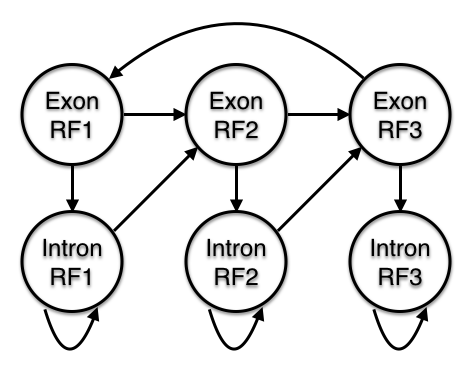
\includegraphics[scale=0.4]{HMM.png}
	\end{center}
	\caption{\label{font-table} Hidden Markov Model for exons and introns.}
\end{figure}

\subsection{Training}
We trained a total of 10 models on 4 different states (orf1, orf2, orf3, intron). These models include: orf1 $\rightarrow$ orf2, orf2 $\rightarrow$ orf1, orf3 $\rightarrow$ orf1, each of the orfs  $\rightarrow$  intron, intron  $\rightarrow$ each of the orfs, and intron  $\rightarrow$  intron. The 3 intron states are all identical (hence why we combined them into a single state here) but we must represent it as 3 states when calculating our model to enforce the reading frame constraint. For each model, we count all the kmers of every length up to the maximum such that the first k-1 bases lie in the first state and the last base lies in the second state.

We trained our model on 10\% of the genes from our dataset. And tested on the remaining 90\%.

\subsection{HIMM}
We used dynamic programming to implement our HIMM. We first construct an empty matrix with 6 rows (one for each state) and a column for each base in the gene to be modeled. We then fill this matrix column by column such that $M_{i,j}$ contains the log-probability of the most likely path from the beginning of the gene to state i for base j. For each state, there are only 2 possible states that can precede it as shown in Figure <<reference>>. We use the Interpolated Markov Model to determine the most likely new state given the preceding kmer and the kmer counts from the training step. The new probability is equal to

$$M_{ij} = \max_{k \in states} M_{k,j-1} \cdot Pr\left({S_\ell}_i \mid \left( S_1,...S_{\ell-1}  \right)_k \right)$$

 In parallel with filling in the probability matrix, we fill in a backtrace matrix of the same dimensions that stores the backtrace of the most likely path from each state to $M_{0,0}$. After completing both matrices, we simply find the highest value in the last column of the probability matrix and follow the backtrace from the corresponding cell in the backtrace matrix.



\section{Results}

As previously mentioned, we are using the complete H. \emph{influenzae} genome to evaluate the performance of our IMM gene classifier. We ran the IMM algorithm under different training and test settings. We evaluated the model performance at maximum k-mer length between the range 0 to 9. A maximum k-mer length of 0 indicates that predictions are made independently of the preceding nucleotide in the DNA sequence, while a maximum k-mer length of 9 indicates that the current nucleotide’s probability is dependent upon at most 9 preceding DNA nucleotides. 

We implemented and tested a fixed-length Markov chain model matching to the order of the IMM in order to compare to our IMM results.

\subsection{Comparison of IMM and Markov chain on H.influenzae data}
Figure 2 shows how the IMM compares against the Markov chain model at identification of H. \emph{influenzae} genes at the different model complexities.

When running our IMM and Markov chain programs, we imposed the same set of selection criteria as the mentioned in the publication. First, we would rule out all ORF’s that are less than 500 bases long, since longer ORF length are more likely to be coding regions. Next, we impose the constraint that the potential ORFs selected must not overlap one another. 

\begin{figure}
	\begin{center}
		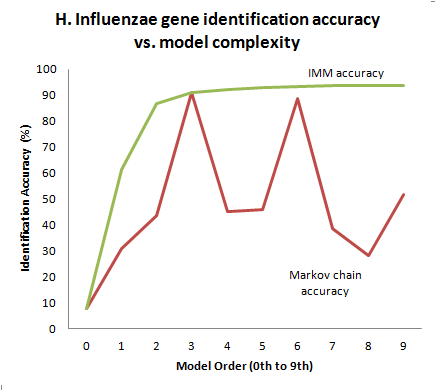
\includegraphics[scale=0.8]{plots/accuracy_vs_model_complexity.png}
	\end{center}
	\caption{\label{font-table} Accuracy comparison for IMM and MC models at different model complexity for \emph{H. influenzae} genome}
\end{figure}

Besides comparing the gene identification accuracies between our models, we chose to record the running time for our models as well. We ran both the IMM and the Markov chain models at different complexities on the H. influenzae genome to generate Figure 3. 

\begin{figure}
	\begin{center}
		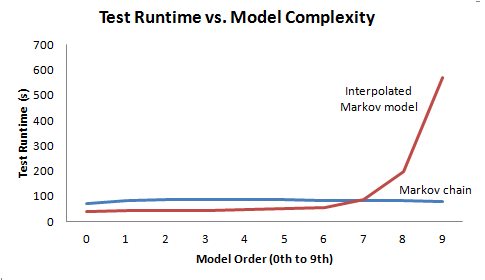
\includegraphics[scale=0.8]{plots/runtime_vs_model_complexity.png}
	\end{center}
	\caption{\label{font-table} Runtime comparison for IMM and MC models at different model complexity}
\end{figure}

We thought checking the number of false positives would be interesting. Figure 4 shows the counts of false positives selected by our models. 

\begin{figure}
	\begin{center}
		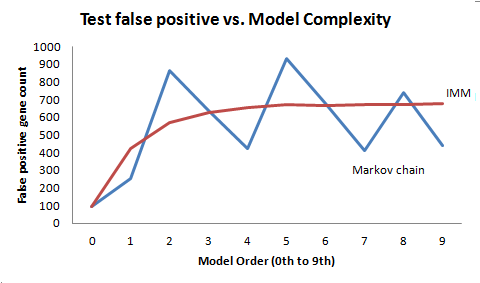
\includegraphics[scale=0.8]{plots/false_positives_vs_model_complexity.png}
	\end{center}
	\caption{\label{font-table} False positive gene identified for IMM and MC models at different model complexity}
\end{figure}

We were interested to see how our model generalize to other bacterial genomes, so we ran similar tests on H. pylori and E.coli genomes. The comparisons between an $8^th$ order interpolated Markov model and an $8^th$ order Markov chain for different prokaryotes are shown in Table 1.

\begin{table}
	\begin{center}
		\begin{tabular}{|c|c|c|}
			\hline \bf Organism & \bf MC Acc.(\%) & \bf IMM Acc.(\%) \\ \hline
			H. influenzae & 51.87 & 93.87 \\
			\hline
			H. pylori & 44.47 & 96.88 \\
			\hline
			E. coli & 27.92 & 58.79 \\
			\hline
		\end{tabular}
	\end{center}
	\caption{\label{font-table} Generalization of Markov chain and interpolated Markov model to other prokaryotic genomes at $9^{th}$ order complexity}
\end{table}


\subsection{Gene finding on Eukaryotic organisms}

While not mentioned in the original GLIMMER publication, gene identification on Eukaryotic genome sequences using the IMM is something we set out to test. Using the complete genome for Drosophila melanogaster’s chromosome X, we ran our IMM and fixed-length Markov chain algorithms to yield the results as shown in Figure 5.

\begin{figure}
	\begin{center}
		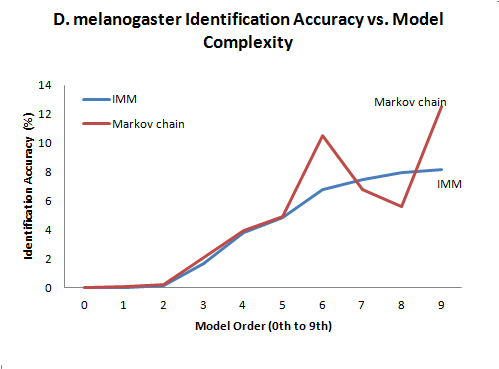
\includegraphics[scale=0.8]{plots/accuracy_vs_model_complexity_drosophila.png}
	\end{center}
	\caption{\label{font-table} Accuracy comparison for IMM and MC models at different model complexity for \emph{D. melanogaster} genome}
\end{figure}

We noticed the poor gene identification accuracy. This result is expected, since Eukaryotic genomes are much more complex than that of Prokaryote’s. For example, the extra non-coding intron sequences and the regulatory sequences such as promoters and enhancers increase the noise which our gene identifier has to go through. 

\subsection{Gene finding on with interpolated Hidden Markov Models}


\begin{figure}
	\begin{center}
		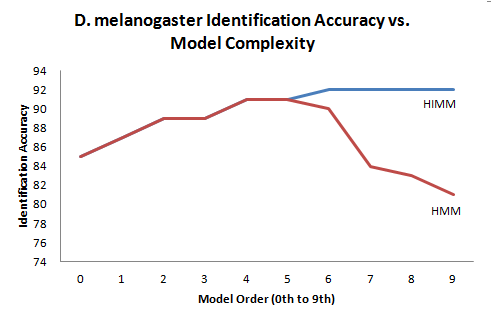
\includegraphics[scale=0.8]{plots/accuracy_vs_model_complexity_drosophila_hmm.png}
	\end{center}
	\caption{\label{font-table} Accuracy comparison for HIMM and HMM models at different model complexity for \emph{D. melanogaster} genome}
\end{figure}


\section{Discussion}

When comparing our 8th order IMM results against the same model as used in the publication, we notice that our accuracy value, of 93.78 \%, differs from the accuracy of 97.8 \% reported. There are several reasons that might have caused this difference.

We noticed there were 1717 annotated genes for the publication while our annotated gene file only contained 1174 genes. We suspect that they had additional experimental data to work with. This difference in the number of annotated genes only affected the number of false positive ORF turn outs in our results. Since we are mainly focused on replicating the results for true positives, we decided to ignore this difference.

From the fixed-length Markov chain results, we noticed that the identification accuracy peaks at intervals of three bases. We think that this might be due to the codon length. 

Overall, we are satisfied with the sensitivity of our IMM on the identification of true bacterial genes.

\subsection{Comparison to Project Proposal}
Judging by our original project proposal, we have accomplished the must-achieve milestones by implementing an IMM classification program closely following the program specifications of the GLIMMER publication. We have also managed to finish the features mentioned in the expected to achieve section. We have written a Markov model to compare the results obtained to that of the IMM’s. If we had additional time, we would likely to have accomplished the reach-goals for improving upon the IMM’s accuracy by training additional model organisms and to implement an interpolated context model to decide which positions to use for prediction.


\begin{thebibliography}{}

\bibitem[\protect\citename{Salzberg, S.L., Delcher, A.L., Kasif, S. and White, O.}1998]{Salzberg:98}
Salzberg, S.L., Delcher, A.L., Kasif, S. and White, O.
\newblock 1998.
\newblock {\em Microbial gene identification using interpolated Markov models}
\newblock Nucleic Acids Research: Oxford University Press.

\bibitem[\protect\citename{Salzberg,S.L., Pertea,M., Delcher,A.L., Gardner,M.J. and
	Tettelin,H.}1999]{}
Salzberg,S.L., Pertea,M., Delcher,A.L., Gardner,M.J. and
Tettelin,H.
\newblock 1999.
\newblock {\em Interpolated Markov models for eukaryotic
	gene finding}
\newblock Genomics, 59, 24–31.

\bibitem[\protect\citename{Henderson, J., Salzberg, S.L., and Fasman K.}1996]{}
Henderson, J., Salzberg, S.L., and Fasman K.
\newblock 1996.
\newblock {\em Finding Genes in DNA with a Hidden Markov Model}
\newblock Journal of Computational Biology.

\end{thebibliography}

\end{document}
